\documentclass[12pt]{article}

% Paquetes necesarios
\usepackage[utf8]{inputenc}
\usepackage[T1]{fontenc}
\usepackage[spanish]{babel}
\usepackage{graphicx}   % imágenes
\usepackage{geometry}   % márgenes
\usepackage{xcolor}     % colores
\usepackage{mdframed}   % recuadros
\usepackage{enumitem}   % listas con control
\usepackage{kantlipsum}   % alineación de texto
\geometry{margin=1.5cm}

% Estilo de recuadro azul para ejercicios
\newmdenv[
  backgroundcolor=blue!10,
  linecolor=blue!50!black,
  linewidth=1pt,
  topline=false, bottomline=false, rightline=false,
  innertopmargin=6pt, innerbottommargin=6pt, innerleftmargin=6pt
]{ejercicio}

\begin{document}

% Encabezado con logos
\begin{center}

    \hrule
    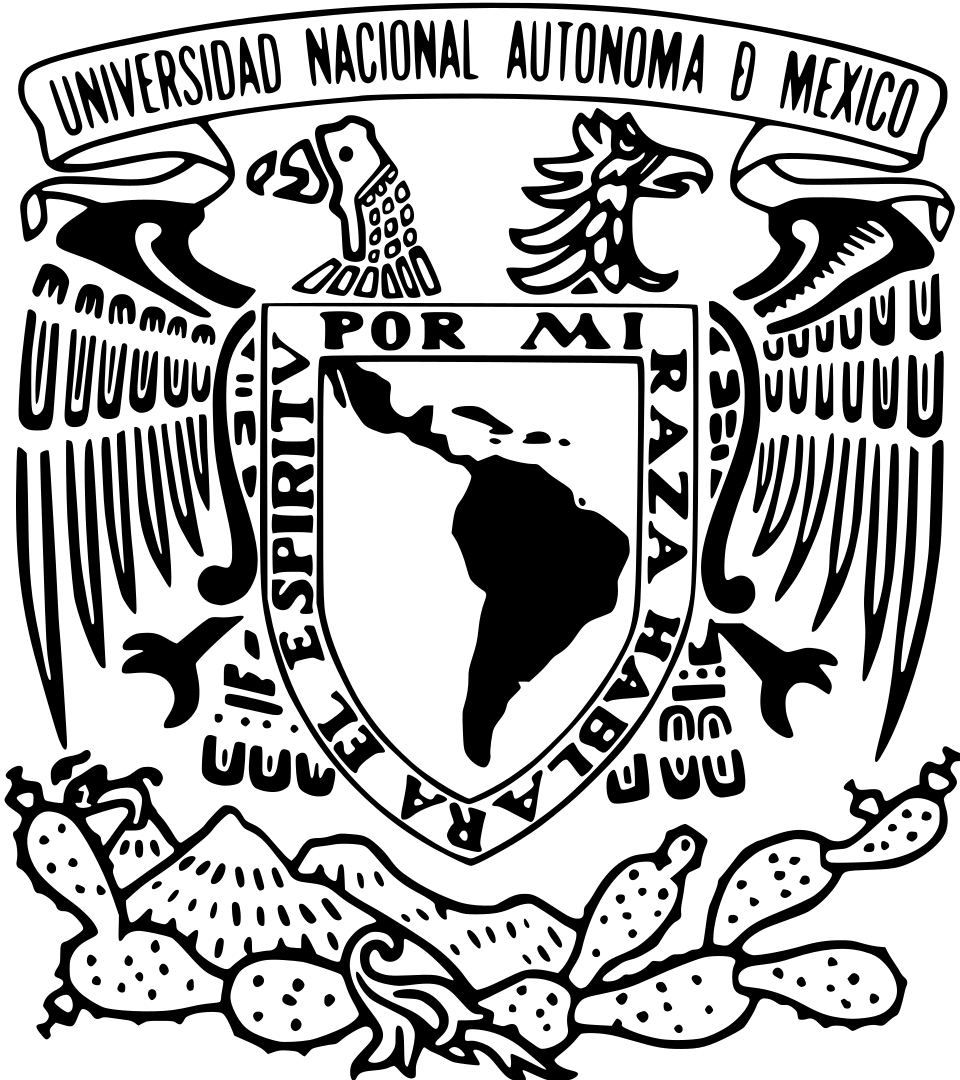
\includegraphics[width=0.1\textwidth]{img/escudo-unam.png}
    \hfill
    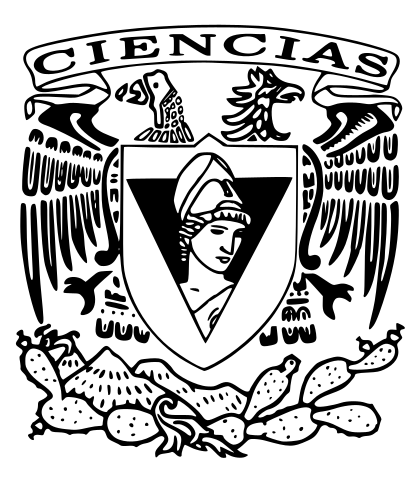
\includegraphics[width=0.1\textwidth]{img/escudo-ciencias.png}
    
    \vspace{-0.5cm}
    
    {\large \textbf{UNIVERSIDAD NACIONAL AUTÓNOMA DE MÉXICO}}\\
    {\medium \textbf{FACULTAD DE CIENCIAS}}\\
    {\medium \textbf{COMPUTACIÓN DISTRIBUIDA}}\\
    {\medium Tarea 1}
\end{center}

\vspace{0.5cm}


\mbox{}\hfill 2026-1

\vspace{0.8cm}

% === EJERCICIOS ===
\begin{ejercicio}
\textbf{Ejercicio 1.} ¿Cuál es la diferencia entre el cómputo concurrente, el cómputo paralelo y el cómputo distribuido?
\end{ejercicio}
\textbf{El cómputo concurrente} divide una tarea en varias partes, y su parte se procesa simultáneamente pero no en el mismo instante. Utiliza una sola unidad de procesamiento.\\
\textbf{El cómputo en paralelo} aumenta la velocidad de cáluclo utilizando múltiples procesos. Divide las tareas en el mismo instante. Utiliza varias unidades de procesamiento.\\
\textbf{El cómputo distribuido} realiza la ejecución de tareas mediante varias computadoras o máquinas conectadas mediante el intercambio de mensajes.
\vspace{0.5cm}
\begin{ejercicio}
\textbf{Ejercicio 2.} ¿Por qué no hay un \textit{único} modelo de cómputo distribuido?
\end{ejercicio}
Porque existen diferentes modelos que reflejan distintas suposiciones sobre la sincronización y la comunicación. Los modelos síncrono y asíncrono son los fundamentales de la computación distribuida, y entre ellos hay varios modelos entre estos extremos. Cada modelo tiene características propias que lo hacen adecuado para distintos tipos de situaciones.
\vspace{0.5cm}
\begin{ejercicio}
\textbf{Ejercicio 3.} ¿Por qué el cómputo distribuido se relaciona a menudo con el término Big Data?
\end{ejercicio}
Porque el cómputo distribuido implica computadoras conectadas que trabajan para resolver un problema en común mediante el intercambio de mensajes. Esta capacidad de cooperación entre permite dividir conjuntos grandes de datos en partes más pequeñas, procesarlas en dispositivos de cómputo individuales que se pueden comunicar entre si y después combinar los resultados reduciendo el tiempo de procesamiento y aprovechando recursos aumentando la eficiencia.\\

\begin{ejercicio}
\textbf{Ejercicio 4.} Explica porqué es posible tener paralelismo sin concurrencia y concurrencia sin paralelismo.
\end{ejercicio}
\textbf{El paralelismo} se concibe con el fin de aumentar la velocidad de cálculo mediante el uso de
múltiples procesos. Es una técnica de ejecución simultánea de diferentes tareas en el mismo
instante. Implica varias unidades de procesamiento independientes que operan en paralelo y
realizan tareas con el fin de aumentar la velocidad de cálculo y mejorar el rendimiento.\\
\textbf{La concurrencia} es una técnica utilizada para disminuir el tiempo de respuesta del sistema que
utiliza una sola unidad de procesamiento o procesamiento secuencial. Una tarea se divide en
varias partes, y su parte se procesa simultáneamente pero no en el mismo instante.
\begin{itemize}
    \item Paralelismo sin concurrencia: Cuando múltiples procesadores trabajan  pero ejecutan una tarea única y independiente al mismo tiempo sin alternarse.
    
    \item Concurrencia sin paralelismo: Cuando una sola unidad de procesamiento alterna entre tareas para simular ejecución simultánea. Como se nos mencionó en clase qu el procesador alterna muy rápidamente pareciendo que hay concurrencia pero solo está ejecutando una instrucción de una sola tarea.
\end{itemize}

\begin{ejercicio}
\textbf{Ejercicio 5.} ¿Cuáles son las diferencias entre un sistema síncrono, un sistema asíncrono, un algoritmo síncrono y un algoritmo asíncrono?
\end{ejercicio}

\begin{itemize}
    \item Sistema síncrono: Los procesadores operan paso a paso ejecutándose en rondas; los mensajes se envían y reciben en la misma ronda.
    \item Sistema asíncrono: No hay reloj global; no hay un limite superior fijo sobre cuanto tiempo tarda en entregar un mensaje o cuanto tiempo transcurre entre los pasos consecutivos de un procesador.
    \item Algoritmo síncrono: Diseñado para sistemas síncronos, los
            procesos se ejecutan colectivamente una secuencia de rondas, se rige por un reloj global externo.
            Los nodos operan en rondas síncronas. \\
            En cada ronda, cada procesador ejecuta los siguientes pasos:\\
            • Realiza algún cálculo local (de complejidad razonable).\\
            • Enviar mensajes a los vecinos de la gráfica (de tamaño razonable).\\
            • Recibir mensajes (enviados por los vecinos en el paso 2 de la misma ronda).
    \item Algoritmo asíncrono: Diseñado para sistemas asíncronos; se rige en eventos y no existe la noción de tiempo externo por lo que no hay un reloj global. Un mensaje enviado de un procesador a otro llegará en un tiempo finito pero ilimitado.\\
    Un proceso procesa un mensaje a la vez. Cuando llega un mensaje,
    se añade al buffer de entrada del proceso receptor. Se procesará después de que se hayan procesado todos los mensajes que le preceden en este buffer.
\end{itemize}

\begin{ejercicio}
\textbf{Ejercicio 6.} ¿El internet es un sistema \textit{síncrono} o \textit{asíncrono}? Justifica tu respuesta.
\end{ejercicio}
Internet es asíncrono, porque no hay un límite superior fijo para el tiempo que tarda la entrega de mensajes ni para los pasos en un procesador.
En internet, el tiempo que tarda un mensaje en viajar desde el origen hasta el destino es variable. Depende de muchísimos factores.
La manera en que funciona internet es como cuando un nodo envía un mensaje y luego se queda esperando hasta que el evento donde llega un mensaje ocurra, cosa que no sabemos cuándo sucederá.
\vspace{0.5cm}
\begin{ejercicio}
\textbf{Ejercicio 7.} ¿Cómo se define la complejidad en tiempo para los algoritmos síncronos?
\end{ejercicio}
Para algoritmos síncronos la complejidad temporal es el número de rondas hasta que el algoritmo termina.  
En cada ronda, cada nodo puede:
\begin{enumerate}
    \item Recibir los mensajes enviados por sus vecinos en la ronda anterior,
    \item Realizar un cómputo local (en tiempo constante), y
    \item Enviar un mensaje a cada uno de sus vecinos.
\end{enumerate}
\begin{ejercicio}
\textbf{Ejercicio 8.} Explica con tus propias palabras el modelo \textbf{LOCAL} y el modelo \textbf{CONGEST}.
\end{ejercicio}
El modelo local se caracteriza por tener importancia en el tiempo que se tarda en ejecutar el número de rondas síncronas hasta que todos los nodos finalizan y puede tener mensajes ilimitados, mientras que en el modelo CONGEST a diferencia de el otro sus mensajes están limitados a O(Log(n)) bits por lo que cada nodo solo puede enviar mensajes pequeños entre cada ronda y es mas realista debido a que simula redes reales donde puede haber congestión debido a que sus canales tienen capacidad limitada.
\vspace{0.5cm}
\begin{ejercicio}
\textbf{Ejercicio 9.} ¿Qué es la contención de nodos?
\end{ejercicio}
En cada paso de un algoritmo síncrono, cada nodo sólo puede enviar y recibir O(1) mensajes que contengan O(1) valores, independientemente del número de vecinos que tenga el nodo.
\vspace{0.5cm}
\begin{ejercicio}
\textbf{Ejercicio 10.} Demuestra el siguiente lema:
\begin{quote}
\textbf{Lema 1.} Una gráfica no dirigida es un árbol si y solo si existe exactamente un camino simple entre cada par de vértices.
\end{quote}
\end{ejercicio}

Recordemos que por definición un \emph{árbol} es una gráfica finita, conexa y acíclica.

\textbf{($\Rightarrow$)} 
Supongamos que $G$ es un árbol. Ahora demostrare que entre cada par de vértices existe exactamente un camino simple. 
Por inducción tenemos que: $n = |V(G)|$.

\emph{Caso base.}  
Si $n=1$, la afirmación es trivial.  
Si $n=2$, el árbol debe consistir en una única arista entre los dos vértices, y dicho camino es único.

\emph{Paso inductivo.}  
Supongamos que la afirmación es cierta para todo árbol de $n-1$ vértices. Sea $G$ un árbol con $n$ vértices ($n \geq 2$).  

Como $G$ es un árbol finito, existe al menos una hoja $v$ (vértice de grado $1$). Sea $u$ el vecino de $v$, y definamos $G' = G - v$ como la gráfica resultante de eliminar $v$ y la arista $uv$.  

Entonces tenemos que: 
\begin{itemize}
    \item $G'$ es un árbol (al quitar una hoja no se destruye la conexidad ni se crea un ciclo).
    \item Por hipótesis inductiva, en $G'$ existe exactamente un camino simple entre cada par de vértices.
\end{itemize}

Ahora, en $G$:
\begin{itemize}
    \item Si los vértices $x,y$ son distintos de $v$, cualquier camino simple entre $x$ y $y$ en $G$ no involucra a $v$, de modo que coincide con el único camino en $G'$.
    \item Si uno de los vértices es $v$ y el otro es $w \neq v$, entonces cualquier camino de $v$ a $w$ debe comenzar con $v u$, seguido del único camino de $u$ a $w$ en $G'$. Por lo tanto existe exactamente un camino simple de $v$ a $w$ en $G$.
\end{itemize}

Así, en todos los casos existe exactamente un camino simple, lo que completa el paso inductivo.  
Por inducción, la afirmación vale para todo árbol $G$.

\bigskip
\textbf{($\Leftarrow$)}  
Supongamos ahora que en $G$ existe exactamente un camino simple entre cada par de vértices.  

\emph{Conexidad.} Por hipótesis, entre cada par de vértices existe al menos un camino, por lo que $G$ es conexa.

\emph{Aciclicidad.} Supongamos que $G$ contiene un ciclo simple $C$. Tomemos dos vértices distintos $x,y$ en $C$.  
En el ciclo existen dos caminos simples distintos entre $x$ e $y$ (recorriendo el ciclo en sentidos opuestos), lo cual contradice la hipótesis de unicidad.  
Por tanto, $G$ no contiene ciclos.

Por lo que $G$ es conexa y acíclica, por lo que $G$ es un árbol.


\vspace{0.5cm}
\begin{ejercicio}
\textbf{Ejercicio 11.} Explica con tus propias palabras el funcionamiento de un algoritmo distribuido que calcule la distancia entre la raíz de una gráfica y el nodo que se está visitando.
\end{ejercicio}

\begin{enumerate}
    \item La raíz comienza enviando un mensaje a todos sus vecinos que sería el siguiente:  
    ``Soy la raíz y mi distancia respecto a ti es 0''.
    
    \item Cada vecino que recibe el mensaje por primera vez:
    \begin{enumerate}
        \item Calcula su distancia como la distancia del emisor + 1.
        \item Guarda esa distancia como la mínima.
        \item Reenvía el mensaje a todos sus propios vecinos.
    \end{enumerate}

    \item Cuando un nodo recibe mas de un mensaje los filtra de la siguiente forma: 
    \begin{enumerate}
        \item Se queda con la distancia más corta.
        \item Ignora los demás porque ya conoce la distancia mínima a la raíz.
    \end{enumerate}
    
    \item Este proceso continúa hasta que todos los nodos han recibido un mensaje desde la raíz.
\end{enumerate}

\begin{ejercicio}
\textbf{Ejercicio 12.} Para el algoritmo propuesto en el ejercicio anterior, argumenta cuántos mensajes es necesario enviar para diseminar el mensaje y cuál es el tamaño de cada mensaje enviado.
\end{ejercicio}
\noindent \textbf{Número de mensajes:} \\
Cada arista de la gráfica transmite un mensaje a lo sumo una vez en cada dirección. 
Por lo tanto, el número total de mensajes es $O(m)$, donde $m$ es el número de aristas de la gráfica. 

\medskip
\noindent \textbf{Tamaño de cada mensaje:} \\
Cada mensaje contiene la identificación de la raíz y la distancia actual. 
Por lo tanto, el tamaño de cada mensaje es $O(\log n)$ bits, donde $n$ es el número de nodos de la gráfica.


 
\end{document}
